\chapter{Introduction}

A computer network is a set of computers sharing resources.
These computers, as well as the network devices interconnecting them, are also called \emph{network nodes}.
The interconnections between these nodes are either made up of physical cables or by using wireless radio frequencies.
Examples of these interconnections include fiber optic cabling, twisted pair, coax, Wi-Fi, Bluetooth, and \abbr{5G}.



\section{The size of a network}

We can categories computer network depending on their geographical size.
A small network spanning a local area, e.g.~a house or office building, is called a \emph{local area network} or \abbr{LAN}.
A large network spanning a country, continent or even the entire world, is called a \emph{wide area network} or \abbr{WAN}.
The networks operated by Internet service providers are such examples but the best known example is of course the Internet itself.

There are several categories in between these two extremes, for example a campus area network (\abbr{CAN}) or metropolitan area network (\abbr{MAN}) but these terms are not that widely used.
The term \abbr{SAN} or \emph{storage area network} is in common use, however, and refers to a network connecting storage appliances together.



\section{Network topologies}

Apart from their physical size we can also categorise networks based on their topology.
There is a difference between the physical topology -- how the cables go -- and the logical topology -- how the data flows through the network.
Let's start off with the most simple topology: a point-to-point link between two devices.
Examples include a serial cable connecting a terminal to the computer, a direct connection using a \abbr{UTP} cable, or an infrared connection.

Next consider the ring topology in \vref{fig:intro-topo-ring}.
Note that this can be considered a series of point-to-point links.
There is a big difference between a ring topology and a series of point-to-point links, however.
Where a series of point-to-point links can still function correctly when one of the links is broken, a ring topology requires the ring to be intact.
This is because the ring topology uses a protocol that passes a token around the ring used for deciding when a host can put data on the ring.
Examples of a ring topology include \abbr{FDDI} and Token Ring, both of which no longer exist.


\begin{figure}
   \centering
   Ring topology
   \caption{Computers connected in a ring topology}
   \label{fig:intro-topo-ring}
\end{figure}


This ring topology can be both a physical and a logical ring, or it could be a physical star topology and a logical ring topology.
An example is Token Ring which has a central \emph{media access unit} (\abbr{MAU}) to which all computers connect.
The \abbr{MAU} makes sure all devices are logically connected in a ring and, when a cable gets disconnected or a device is turned off, the \abbr{MAU} skips that link and restores the ring with the remaining devices.

Both Thicknet and Thinnet form a physical and logical bus topology (\vref{fig:intro-topo-bus}) with all devices connecting to a long cable.
Ethernet hubs form a physical star topology with the hub being the centre, much like the \abbr{MAU} in a Token Ring network.
Logically the Ethernet network operates just like the Thinnet bus topology as all devices receive all traffic on the wire.
An Ethernet switch changes this behavior as it isolates the differnet cable segments from each other.
It thus forms both a physical and a logical star topology.


\begin{figure}
   \centering
   Bus topology
   \caption{Computers connected in a bus topology}
   \label{fig:intro-topo-bus}
\end{figure}

A mesh topology interconnects all devices with each other.
A \emph{full mesh} (\vref{fig:intro-topo-full-mesh}) connects every device with every other device while in a \emph{partial mesh} (\vref{fig:intro-topo-partial-mesh}) some of the connections are missing.


\begin{figure}
   \begin{subfigure}[b]{.47\textwidth}
      \centering
      FULL MESH
      \caption{A full mesh}
      \label{fig:intro-topo-full-mesh}
   \end{subfigure}
   \hfill
   \begin{subfigure}[b]{.47\textwidth}
      \centering
      PARTIAL MESH
      \caption{A partial mesh}
      \label{fig:intro-topo-partial-mesh}
   \end{subfigure}
   \caption{Meshed networks}
   \label{fig:intro-topo-mesh}
\end{figure}


%Thick- en thinnet gebruiken beide een fysieke busstructuur waarbij alle computers op één lange kabel geprikt worden.
%Beide standaarden gebruiken coax (echter van een andere dikte, vandaar de namen) maar beide gebruiken een andere manier om de computers met het netwerk te verbinden.
%Thicknet gebruikt ``vampire taps'' en een \emph{drop cable} terwijl thinnet BNC-koppelstukken gebruikt.%
%   \footnote{Er was ook een N-connector beschikbaar voor Thicknet maar deze werd blijkbaar amper gebruikt (\href{http://www.mattmillman.com/projects/10base5/}{bron}).}



\section{Network protocols}

A communication protocol is a system of rules that allows two or more entities of a communications system to transmit information.
The protocol defines the rules, syntax, semantics and synchronization of communication and possible error recovery methods.
Protocols may be implemented by hardware, software, or a combination of both.

Multiple protocols often describe different aspects of a single communication.
A group of protocols designed to work together is known as a \emph{protocol suite}; when implemented in software they are a \emph{protocol stack}.

Some of the protocols we will (briefly) cover in this course are \abbr{IP} versions~4 and~6, \abbr{TCP}, \abbr{UDP}, Ethernet, and \abbr{ARP}.
Some of the network protocols which are no longer in use, include \abbr{IPX} and AppleTalk.



\section{A brief history of computer networks}

The first \emph{mainframes} appeared in the fifties.
Data had to be entered using punched cards or mangetic tape.
Output had to be printed as there were no monitors yet.
You first had to load the program into memory and then the date you wished to process.
There were no operating systems yet.
It wasn't until the early seventies when terminals were being used.

\begin{itemize}
\item
   In the late 1950s, a network of computers was built for the U.S. military semi-automatic ground environment (\abbr{SAGE}) radar system using the Bell 101 modem.
   It was the first commercial modem for computers, released by AT\&T Corporation in 1958.
   The modem allowed digital data to be transmitted over regular unconditioned telephone lines at a speed of 110 bits per second~(bit/s).
\item
   In 1959, Christopher Strachey filed a patent application for time-sharing and John McCarthy initiated the first project to implement time-sharing of user programs at MIT.
   Stratchey passed the concept on to J. C. R. Licklider at the inaugural \abbr{UNESCO} Information Processing Conference in Paris that year.
   McCarthy was instrumental in the creation of three of the earliest time-sharing systems (Compatible time-sharing system in 1961, BBN time-sharing system in 1962, and Dartmouth time sharing system in 1963).
\item
   In 1959, Anatoly Kitov proposed to the Central Committee of the Communist Party of the Soviet Union a detailed plan for the re-organisation of the control of the Soviet armed forces and of the Soviet economy on the basis of a network of computing centres.
   Kitov's proposal was rejected, as later was the 1962 OGAS economy management network project.
\item
   In 1960, the commercial airline reservation system semi-automatic business research environment (\abbr{SABRE}) went online with two connected mainframes.
\item
   In 1963, J. C. R. Licklider sent a memorandum to office colleagues discussing the concept of the ``Intergalactic Computer Network,'' a computer network intended to allow general communications among computer users.
\item
   Throughout the 1960s, Paul Baran and Donald Davies independently developed the concept of packet switching to transfer information between computers over a network.
   Davies pioneered the implementation of the concept.
   The \abbr{NPL} network, a local area network at the National Physical Laboratory (United Kingdom) used a line speed of 768 kbit/s and later high-speed T1 links (1.544 Mbit/s line rate).
\item
   In 1965, Western Electric introduced the first widely used telephone switch that implemented computer control in the switching fabric.
\item
   In 1969, the first four nodes of the \abbr{ARPANET} were connected using 50 kbit/s circuits between the University of California at Los Angeles, the Stanford Research Institute, the University of California at Santa Barbara, and the University of Utah.
   In the early 1970s, Leonard Kleinrock carried out mathematical work to model the performance of packet-switched networks, which underpinned the development of the \abbr{ARPANET}.
   His theoretical work on hierarchical routing in the late 1970s with student Farouk Kamoun remains critical to the operation of the Internet today.
\item
   In 1972, commercial services were first deployed on public data networks in Europe, which began using X.25 in the late 1970s and spread across the globe.
   The underlying infrastructure was used for expanding \abbr{TCP}/\abbr{IP} networks in the 1980s.
\item
   In 1973, the French \abbr{CYCLADES} network was the first to make the hosts responsible for the reliable delivery of data, rather than this being a centralized service of the network itself.
\item
   In 1973, Robert Metcalfe wrote a formal memo at Xerox \abbr{PARC} describing Ethernet, a networking system that was based on the Aloha network, developed in the 1960s by Norman Abramson and colleagues at the University of Hawaii.
   In July 1976, Robert Metcalfe and David Boggs published their paper ``Ethernet: distributed packet switching for local computer networks'' and collaborated on several patents received in 1977 and 1978.
\item
   In 1974, Vint Cerf, Yogen Dalal, and Carl Sunshine published the Transmission Control Protocol (\abbr{TCP}) specification, \abbr{RFC} 675, coining the term Internet as a shorthand for internetworking.
\item
   In 1976, John Murphy of Datapoint Corporation created \abbr{ARCNET}, a token-passing network first used to share storage devices.
\item
   In 1977, the first long-distance fiber network was deployed by \abbr{GTE} in Long Beach, California.
\item
   In 1977, Xerox Network Systems (\abbr{XNS}) was developed by Robert Metcalfe and Yogen Dalal at Xerox.
\item
   In 1979, Robert Metcalfe pursued making Ethernet an open standard.
\item
   In 1980, Ethernet was upgraded from the original 2.94 Mbit/s protocol to the 10~Mbit/s protocol, which was developed by Ron Crane, Bob Garner, Roy Ogus, and Yogen Dalal.
\item
   In 1995, the transmission speed capacity for Ethernet increased from 10~Mbit/s to 100~Mbit/s.
   By 1998, Ethernet supported transmission speeds of 1~Gbit/s.
   Subsequently, higher speeds of up to 400 Gbit/s were added (as of 2018).
   The scaling of Ethernet has been a contributing factor to its continued use.
\end{itemize}



\section{The \abbr{OSI} and \abbr{TCP}/\abbr{IP} models}

The Open Systems Interconnection (\abbr{OSI}) model is a conceptual model that was developed in the late 1970's for the field of computer networking, and then became an operating model in the 1980's through the International Organization for Standardization (\abbr{ISO}).


Het OSI-model is een conceptueel model voor netwerkcommunicatie.
Het werd als theoretisch model ontwikkeld met de bedoeling dat de praktijk zich aan dit model aan zou passen.
Het TCP/IP-model is een alternatief protocol dat gebaseerd is op de protocollen die al in de praktijk gebruikt werden.

\begin{table}[htp]
   \centering
   \begin{tabular}{rll}
   %\toprule
              & \textsc{osi-model}           & \textsc{tcp/ip-model} \\[1ex]
   %\midrule
   \textit{7} & application                  & \multirow{3}{*}{\textcolor{spot1}{application}} \\
   \textit{6} & presentation                 & \\
   \textit{5} & session                      & \\[1ex]
   \textit{4} & \textcolor{spot1}{transport} & transport \\[1ex]
   \textit{3} & \textcolor{spot1}{network}   & internet \\[1ex]
   \textit{2} & \textcolor{spot1}{data link} & \multirow{2}{*}{link} \\
   \textit{1} & \textcolor{spot1}{physical}  & \\
   %\bottomrule
   \end{tabular}
   \caption{De zeven lagen van het OSI-model en de vier lagen van het TCP/IP-model.
   De vijf lagen van het hybride model zijn in kleur weergegeven.}
   \label{tab:osi-model}
\end{table}

Deze modellen hebben weinig praktisch nut maar kunnen wel helpen met het gestructureerd opsporen en oplossen van netwerkproblemen.
Afhankelijk van het probleem kan je ofwel op laag~7 (de applicatie) beginnen met troubleshooten, ofwel op laag~1 (de bekabeling), ofwel in het midden op laag~3 (het netwerk).
Onderstaand vind je voor de vijf lagen van het hybride model enkele zaken die onderzocht kunnen worden.

\begin{description}
\item[application]
   Controleer de configuratie van de applicatie zelf.
   Dit is aan de applicatie- of systeembeheerders en niet aan de netwerkbeheerder.
\item[transport]
   Controleer firewallconfiguraties en of de service (applicatie) wel gestart is op de server.
   Je kan met behulp van \cmd{telnet} testen of de applicatie bereikbaar is.
\item[network]
   Verifiëer met behulp van \cmd{ping} en \cmd{traceroute} of de twee computers elkaar kunnen bereiken.
   De output van \cmd{traceroute} geeft een indicatie hoe de pakketjes doorheen het netwerk gaan.
   Dit kan je best in beide richtingen controleren aangezien \emph{asymetrisch} netwerkverkeer mogelijk is en mogelijk voor problemen kan zorgen.
\item[data link]
   Op het lokale netwerk moet je zaken zoals Spanning-tree protocol (STP) en VLAN-configuraties nakijken.
   Zaken zoals DHCP snooping, dynamic ARP inspection (DAI) en port security kan je hier ook nakijken.
\item[physical]
  Controleer bekabeling, connectors, interface errors en, in het geval van wifi, mogelijke storingsbronnen.
\end{description}

De verschillende lagen vinden we ook terug als we de verschillende stappen doorlopen die computers doorlopen om met elkaar te communiceren.




\section{Routing schemes}

There are four different routing schemes, or ways to deliver a packet on the network.
\begin{description}
\item[unicast] Unicast delivers a message to a single specific node using a one-to-one association between a sender and destination: each destination address uniquely identifies a single receiver endpoint.
\item[broadcast] Broadcast delivers a message to all nodes in the network using a one-to-all association; a single datagram (or packet) from one sender is routed to all of the possibly multiple endpoints associated with the broadcast address. The network automatically replicates datagrams as needed to reach all the recipients within the scope of the broadcast, which is generally an entire network subnet.
\item[multicast] Multicast delivers a message to a group of nodes that have expressed interest in receiving the message using a one-to-many-of-many or many-to-many-of-many association; datagrams are routed simultaneously in a single transmission to many recipients. Multicast differs from broadcast in that the destination address designates a subset, not necessarily all, of the accessible nodes.
\item[anycast] Anycast delivers a message to any one out of a group of nodes, typically the one nearest to the source using a one-to-one-of-many as\-so\-ci\-a\-tion where datagrams are routed to any single member of a group of potential receivers that are all identified by the same destination address. The routing algorithm selects the single receiver from the group based on which is the nearest according to some distance or cost measure.
\end{description}
We will not cover multicast or anycast in this course.



\section{Communication between computers}



Nemen we als voorbeeld een computer, de \emph{client}, die een webpagina op wil halen van een andere computer, de \emph{server} (\vref{fig:client-server}).
Het protocol dat hier voor gebruikt wordt, heet hypertext transfer protocol (HTTP).
De client verstuurt een HTTP \emph{request} en de server antwoordt met een HTTP \emph{response}.

De request bevat de volgende data.
\begin{verbatim}
GET /index.html HTTP/1.1
Host: www.example.com
\end{verbatim}

\begin{figure}
   \centering
   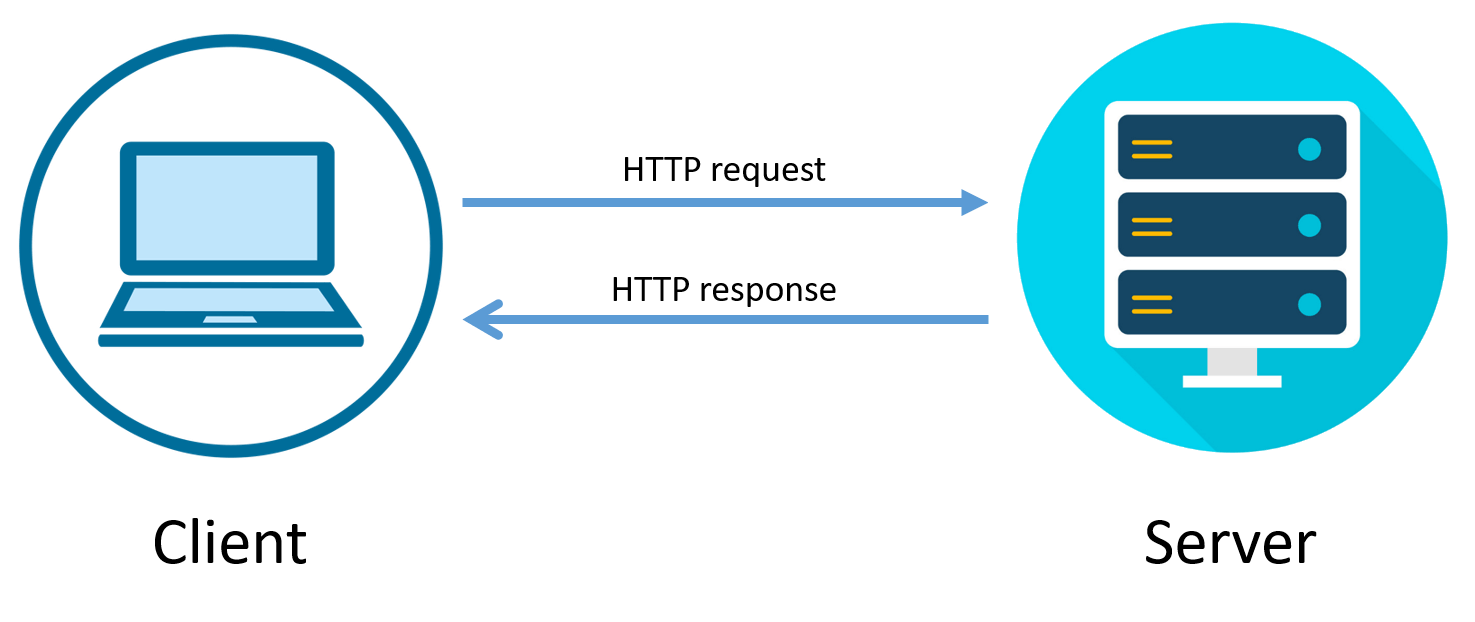
\includegraphics[width=.65\textwidth]{images/http-request.png}
   \caption{Een client vraagt een webpagina op bij eeen webserver en gebruikt voor deze communicatie HTTP}
   \label{fig:client-server}
\end{figure}

Het antwoord van de server bevat enerzijds de HTTP-data die het protocol vereist en anderzijds de gevraagde webpagina.
In dit geval bevat de gevraagde pagina HTML-code.
\begin{verbatim}
HTTP/1.1 200 OK
Content-Type: text/html; charset=UTF-8
Content-Length: 155
Server: Apache/1.3.3.7 (Unix) (Red-Hat/Linux)

<html>
  <head><title>An Example Page</title></head>
  <body><p>Hello World!</p></body>
</html>
\end{verbatim}

Dit ogenschijnlijk eenvoudig voorbeeld roept toch meerdere vragen op.
\begin{enumerate}
\item Hoe kunnen we de server bereiken?
\item Voor welke applicatie is de data bestemd?
\item Hoe versturen we heel veel data?
\item Wat doen we als er iets mis gaat?
\end{enumerate}



\subsection{Hoe kunnen we de server bereiken?}
In de adresbalk van de browser vullen we de \emph{domeinnaam} van de website in die we willen bereiken, bijvoorbeeld \url{www.example.com}.
Deze domeinnaam vinden we ook terug in de Host header van de HTTP request.
Omdat computers met elkaar communiceren door middel van IP-adressen, moet deze domeinnaam eerst omgezet worden in een IP-adres.
Dit gebeurt met behulp van het Domain Name System (DNS).

\subsection{Voor welke applicatie is de data bestemd?}
Als pakketjes aankomen op een server of client computer, moet het besturingssysteem weten voor welke applicatie ze bestemd zijn.
Bevatten de pakketjes een email bestemd voor Outlook of een gif van een kat die in de browser getoond moet worden?
Elk programma dat communiceert op het netwerk krijgt een poortnummer toegewezen.
Deze poortnummers worden meegestuurd in de pakketjes zodat de computers steeds weten voor welke applicatie de pakketjes bestemd zijn.
We leren meer over deze poortnummers als we TCP en UDP bespreken.

\subsection{Hoe versturen we heel veel data?}
Als we een groot document door willen sturen, reist de vraag of we dit document als één geheel kunnen sturen, of moeten opsplitsen in kleine stukjes om vervolgens deze kleine stukjes afzonderlijk te versturen.
We zullen merken dat er technische beperkingen zijn die de maximale grootte van een pakket bepalen op sommige netwerken.
Het is soms dus noodzakelijk om grote bestanden op te splitsen en als kleine stukjes te versturen.

Als we een groot bestand opsplitsen in twintig kleine stukjes en deze afzonderlijk versturen, moet de ontvanger van deze twintig pakketjes er wel in slagen om ze alle twintig terug samen te puzzelen tot één geheel.
De ontvanger moet ook zeker dat dat hij alle stukjes ontvangen heeft.
Het is belangrijk dat hij weet dat de verzender twintig pakketjes verstuurd heeft in plaats van eenentwintig.

Deze vraagt hangt ook samen met de volgende vraag.

\subsection{Wat doen we als er iets mis gaat?}
Pakketjes kunnen verloren gaan of er kunnen ``beschadigingen'' optreden in een pakketje (een ``1'' kan een ``0'' worden of omgekeerd).
Pakketjes kunnen in de verkeerde volgorde aankomen.
Dit zijn uitdagingen die TCP en UDP wel (of bewust niet) oplost.




\section{Encapsulatie en decapsulatie}

We gaan nu terug naar de computer die een HTTP request stuurt naar de web server.
De computer heeft een DNS request uitgestuurd voor de domeinnaam www.example.com en kreeg het IP-adres 192.168.1.102.
De HTTP request wordt nu ``ingepakt'' in een TCP-pakket (\vref{fig:transmit-data}).
Dit ``inpakken'' (\emph{encapsulation}) is niet meer dan wat extra data toe te voegen, ofwel voor ofwel na de andere data.
TCP voegt onder andere de nodige poortnummers toe.


\begin{figure}
   \centering
   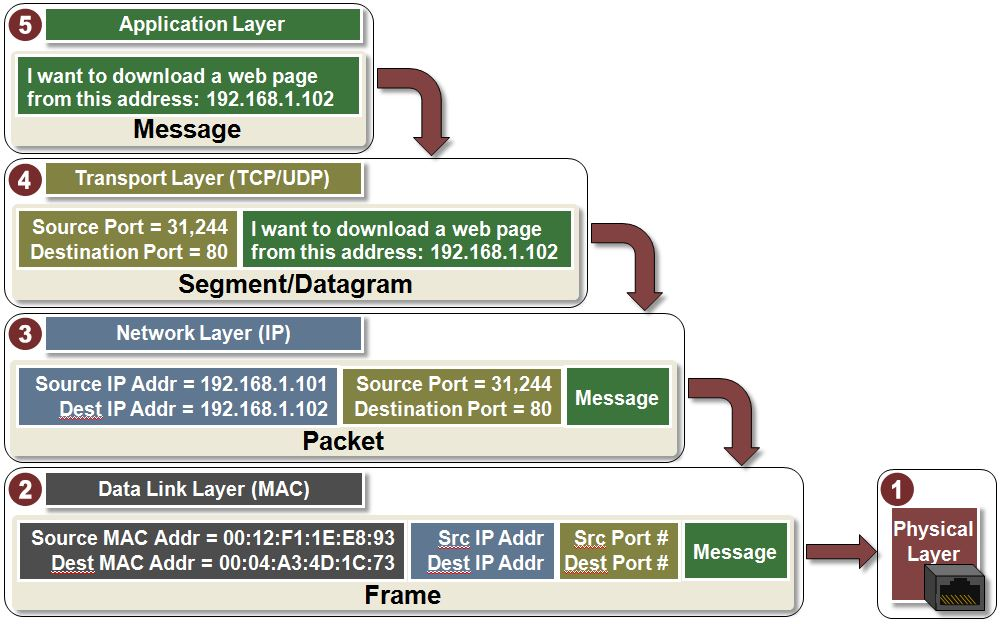
\includegraphics[width=\textwidth]{images/transmit_data.jpg}
   \caption{Elk protocol voegt een eigen header toe aan het pakket}
   \label{fig:transmit-data}
\end{figure}

Vervolgens wordt het pakket doorgegeven aan IP.
Deze voegt de source en destination IP-adressen toe.
Vervolgens voegt Ethernet een header toe met source en destination MAC-adressen waarna het pakket door de netwerkkaart het netwerk wordt opgestuurd.
Dit is de physical layer.


%\begin{frame}{Communicatie gebeurt tussen lagen onderling}
%\begin{center}
%\includegraphics<presentation>[width=\textwidth]{images/tcpip_5_layer_overview.png}
%\includegraphics<article>[width=.65\textwidth]{images/tcpip_5_layer_overview.png}
%\end{center}
%Bron: \url{https://microchipdeveloper.com/}
%\end{frame}
%




\section{Network icons}
